% questions.tex —— 2008 年·普通高等学校招生考试·浙江卷·文科 · 题目内容片段（无答案）
% 由 tools/generate_projects.py 依来源总账自 2008/2008_数学真题_浙江文_试题.md 生成，勿手改（改源 MD 后重跑）


\gkpart{一、选择题}

\begin{question}
\gkti{1}已知集合 $A=\{x\mid x>0\}$，$B=\{x\mid -1\leqslant x\leqslant2\}$，则 $A\cup B=$（　）

（A）$\{x\mid x\geqslant-1\}$

（B）$\{x\mid x\leqslant2\}$

（C）$\{x\mid 0<x\leqslant2\}$

（D）$\{x\mid -1\leqslant x\leqslant2\}$

\end{question}
\begin{question}
\gkti{2}函数 $y=(\sin x+\cos x)^2+1$ 的最小正周期是（　）

（A）$\dfrac{\pi}2$

（B）$\pi$

（C）$\dfrac{3\pi}2$

（D）$2\pi$

\end{question}
\begin{question}
\gkti{3}已知 $a$，$b$ 都是实数，那么“$a^2>b^2$”是“$a>b$”的（　）

（A）充分而不必要条件

（B）必要而不充分条件

（C）充分必要条件

（D）既不充分也不必要条件

\end{question}
\begin{question}
\gkti{4}已知 $\{a_n\}$ 是等比数列，$a_2=2$，$a_5=\dfrac14$，则公比 $q=$（　）

（A）$-\dfrac12$

（B）$-2$

（C）$2$

（D）$\dfrac12$

\end{question}
\begin{question}
\gkti{5}已知 $a\geqslant0$，$b\geqslant0$，且 $a+b=2$，则（　）

（A）$ab\leqslant\dfrac12$

（B）$ab\geqslant\dfrac12$

（C）$a^2+b^2\geqslant2$

（D）$a^2+b^2\leqslant3$

\end{question}
\begin{question}
\gkti{6}在 $(x-1)(x-2)(x-3)(x-4)(x-5)$ 的展开式中，含 $x^4$ 的项的系数是（　）

（A）$-15$

（B）$85$

（C）$-120$

（D）$274$

\end{question}
\begin{question}
\gkti{7}在同一平面直角坐标系中，函数 $y=\cos\left(\dfrac x2+\dfrac{3\pi}2\right)$（$x\in[0,2\pi]$）的图象和直线 $y=\dfrac12$ 的交点个数是（　）

（A）$0$

（B）$1$

（C）$2$

（D）$4$

\end{question}
\begin{question}
\gkti{8}若双曲线 $\dfrac{x^2}{a^2}-\dfrac{y^2}{b^2}=1$ 的两个焦点到一条准线的距离之比为 $3:2$，则双曲线的离心率是（　）

（A）$3$

（B）$5$

（C）$\sqrt3$

（D）$\sqrt5$

\end{question}
\begin{question}
\gkti{9}对两条不相交的空间直线 $a$ 与 $b$，必存在平面 $\alpha$，使得（　）

（A）$a\subset\alpha$，$b\subset\alpha$

（B）$a\subset\alpha$，$b\parallel\alpha$

（C）$a\perp\alpha$，$b\perp\alpha$

（D）$a\subset\alpha$，$b\perp\alpha$

\end{question}
\begin{question}
\gkti{10}若 $a\geqslant0$，$b\geqslant0$，且当 $\begin{cases}x\geqslant0,\\ y\geqslant0,\\ x+y\leqslant1\end{cases}$ 时，恒有 $ax+by\leqslant1$，则以 $a$，$b$ 为坐标的点 $P(a,b)$ 所形成的平面区域的面积是（　）

（A）$\dfrac12$

（B）$\dfrac{\pi}4$

（C）$1$

（D）$\dfrac{\pi}2$

\end{question}
\gkpart{二、填空题}

\begin{question}
\gkti{11}已知函数 $f(x)=x^2+|x-2|$，则 $f(1)=$\gkblank{}。

\end{question}
\begin{question}
\gkti{12}若 $\sin\left(\dfrac{\pi}2+\theta\right)=\dfrac35$，则 $\cos2\theta=$\gkblank{}。

\end{question}
\begin{question}
\gkti{13}已知 $F_1$，$F_2$ 为椭圆 $\dfrac{x^2}{25}+\dfrac{y^2}9=1$ 的两个焦点，过 $F_1$ 的直线交椭圆于 $A$，$B$ 两点。若 $|F_2A|+|F_2B|=12$，则 $|AB|=$\gkblank{}。

\end{question}
\begin{question}
\gkti{14}在 $\triangle ABC$ 中，角 $A$，$B$，$C$ 所对的边分别为 $a$，$b$，$c$，若 $(\sqrt3b-c)\cos A=a\cos C$，则 $\cos A=$\gkblank{}。

\Needspace{0.4\textheight}
\end{question}
\begingroup
\renewenvironment{question}{\Needspace{0.46\textheight}}{}
\begin{question}
\gkti{15}如图，已知球 $O$ 的面上四点 $A$，$B$，$C$，$D$，$DA\perp$ 平面 $ABC$，$AB\perp BC$，$DA=AB=BC=\sqrt3$，则球 $O$ 的体积等于\gkblank{}。
\nopagebreak[4]
\begin{center}% 2008 年浙江卷文科第 15 题：球 O 的面上四点 A、B、C、D，DA⊥平面 ABC，AB⊥BC，
%   DA=AB=BC=√3。
% 来源 PDF：gaokaomath-src/普通高考/2008/2008浙江文.pdf
% SHA-256：751204c132deb2b2...
% 原页：2008浙江文.pdf 第 1 页（A3 三栏）第 2 栏，书页码 493。
% 重绘依据：D 在 A 的正上方（DA 竖直），B 在 A 左下、C 在 B 左侧，AB⊥BC；
%   可见棱 DA、DB、DC、AB、BC 实线，被遮挡的底面斜边 CA 虚线。
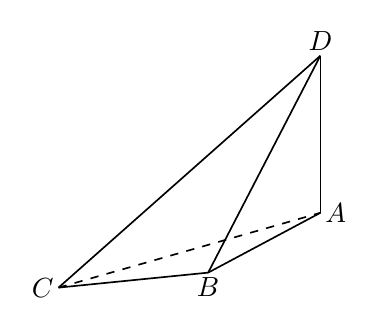
\begin{tikzpicture}[scale=0.95, semithick, every node/.style={inner sep=1.5pt}]
  \coordinate (D) at (5.0,4.7);
  \coordinate (A) at (5.0,2.6);
  \coordinate (B) at (3.5,1.8);
  \coordinate (C) at (1.5,1.6);

  \draw (D) -- (A);
  \draw (D) -- (B);
  \draw (D) -- (C);
  \draw (A) -- (B) -- (C);
  \draw[dashed] (C) -- (A);

  \node[above] at (D) {$D$};
  \node[right] at (A) {$A$};
  \node[below] at (B) {$B$};
  \node[left] at (C) {$C$};
\end{tikzpicture}
\end{center}
\nopagebreak[4]
\end{question}
\endgroup
\begin{question}
\gkti{16}已知 $\boldsymbol a$ 是平面内的单位向量，若向量 $\boldsymbol b$ 满足 $\boldsymbol b\cdot(\boldsymbol a-\boldsymbol b)=0$，则 $|\boldsymbol b|$ 的取值范围是\gkblank{}。

\end{question}
\begin{question}
\gkti{17}用 $1,2,3,4,5,6$ 组成六位数（没有重复数字），要求任何相邻两个数字的奇偶性不同，且 $1$ 和 $2$ 相邻，这样的六位数的个数是\gkblank{}。（用数字作答）

\end{question}
\gkpart{三、解答题}

\begin{question}
\gkti{18}已知数列 $\{x_n\}$ 的首项 $x_1=3$，通项 $x_n=2^np+nq$（$n\in\mathbf N^*$，$p$，$q$ 为常数），且 $x_1$，$x_4$，$x_5$ 成等差数列。求：

（1）$p$，$q$ 的值；

（2）数列 $\{x_n\}$ 前 $n$ 项和 $S_n$ 的公式。

\end{question}
\begin{question}
\gkti{19}一个袋中装有大小相同的黑球、白球和红球，已知袋中共有 $10$ 个球，从中任意摸出 $1$ 个球，得到黑球的概率是 $\dfrac25$；从中任意摸出 $2$ 个球，至少得到 $1$ 个白球的概率是 $\dfrac79$。求：

（1）从中任意摸出 $2$ 个球，得到的数是黑球的概率；

（2）袋中白球的个数。

\Needspace{0.4\textheight}
\end{question}
\begingroup
\renewenvironment{question}{\Needspace{0.5\textheight}}{}
\begin{question}
\gkti{20}如图，矩形 $ABCD$ 和梯形 $BEFC$ 所在平面互相垂直，$BE\parallel CF$，$\angle BCF=\angle CEF=90^\circ$，$AD=\sqrt3$，$EF=2$。

（1）求证：$AE\parallel$ 平面 $DCF$；

（2）当 $AB$ 的长为何值时，二面角 $A-EF-C$ 的大小为 $60^\circ$？
\nopagebreak[4]
\begin{center}% 2008 年浙江卷文科第 20 题：矩形 ABCD 与梯形 BEFC 所在平面互相垂直，BE∥CF，
%   ∠BCF=∠CEF=90°，AD=√3，EF=2。
% 来源 PDF：gaokaomath-src/普通高考/2008/2008浙江文.pdf
% SHA-256：751204c132deb2b2f856ffeba082ce94063aa6e279783c2f07e4cd84539ecb63
% 原页：2008浙江文.pdf 第 2 页（A3 三栏）第 1 栏，书页码 494。
% 重绘依据：按斜投影作图，保持 AB∥DC、AD∥BC、BE∥CF；A 左上、B 左下、D 右上、C 居中、
%   E 在中下、F 在右下；可见棱 AB、AD、AC、AE、AF、DF、BE、EF 实线，自 C 出发的
%   BC、CD、CE、CF 被遮挡用虚线。
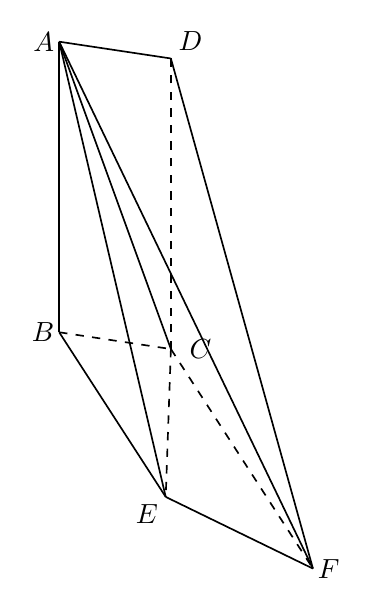
\begin{tikzpicture}[scale=0.82, semithick, every node/.style={inner sep=1.5pt}]
  \coordinate (A) at (1.00,8.50);
  \coordinate (B) at (1.00,4.00);
  \coordinate (C) at (2.73,3.74);
  \coordinate (D) at (2.73,8.24);
  \coordinate (E) at (2.65,1.45);
  \coordinate (F) at (4.93,0.34);

  % 可见棱
  \draw (A) -- (B);
  \draw (A) -- (D);
  \draw (A) -- (C);
  \draw (A) -- (E);
  \draw (A) -- (F);
  \draw (D) -- (F);
  \draw (B) -- (E);
  \draw (E) -- (F);

  % 被遮挡的棱（自 C 出发）
  \draw[dashed] (B) -- (C);
  \draw[dashed] (C) -- (D);
  \draw[dashed] (C) -- (E);
  \draw[dashed] (C) -- (F);

  \node[left] at (A) {$A$};
  \node[left] at (B) {$B$};
  \node[right=5pt] at (C) {$C$};
  \node[above right=1pt] at (D) {$D$};
  \node[below left=1pt] at (E) {$E$};
  \node[right] at (F) {$F$};
\end{tikzpicture}
\end{center}
\nopagebreak[4]
\end{question}
\endgroup
\begin{question}
\gkti{21}已知 $a$ 是实数，函数 $f(x)=x^2(x-a)$。

（1）若 $f'(1)=3$，求 $a$ 的值及曲线 $y=f(x)$ 在点 $(1,f(1))$ 处的切线方程；

（2）求 $f(x)$ 在区间 $[0,2]$ 上的最大值。

\end{question}